\section{Experimental Design}

This section specifies how the methodological framework was operationalized and tested to answer RQ1, RQ2, and RQ3 on the OULAD dataset. Its purpose is to define the evaluation protocol actually used, the fixed comparison rules adopted before inspecting comparative outcomes, and the evidence contract linking claims to metrics and exported artifacts. By the end of the section, the reader should expect a clear description of the cohort construction, split logic, model variants, evaluation horizons, robustness plan, and reading criteria under which the empirical results are interpreted.

This section follows the same narrative structure as the implemented pipeline. It begins with the design goals and analytical units, then defines the split and model tracks, next establishes the censoring-aware evaluation horizons and metric suite, and finally specifies the policy, subgroup, robustness, and traceability protocols. Throughout, the design is presented as a pre-specified experimental framework for evaluating \textit{model-implied simulated regime contrasts}, not as a causal identification strategy for intervention effects.

Figure~\ref{fig:pipeline_endtoend} provides an end-to-end overview of the evaluation tracks.

% Placeholder for compiled Graphviz figure (G1 pipeline_endtoend)
% To produce this figure: dot -Tpng graphviz_pipeline_endtoend.txt -o figures/fig_pipeline_endtoend.png
\begin{figure}[!t]
\centering
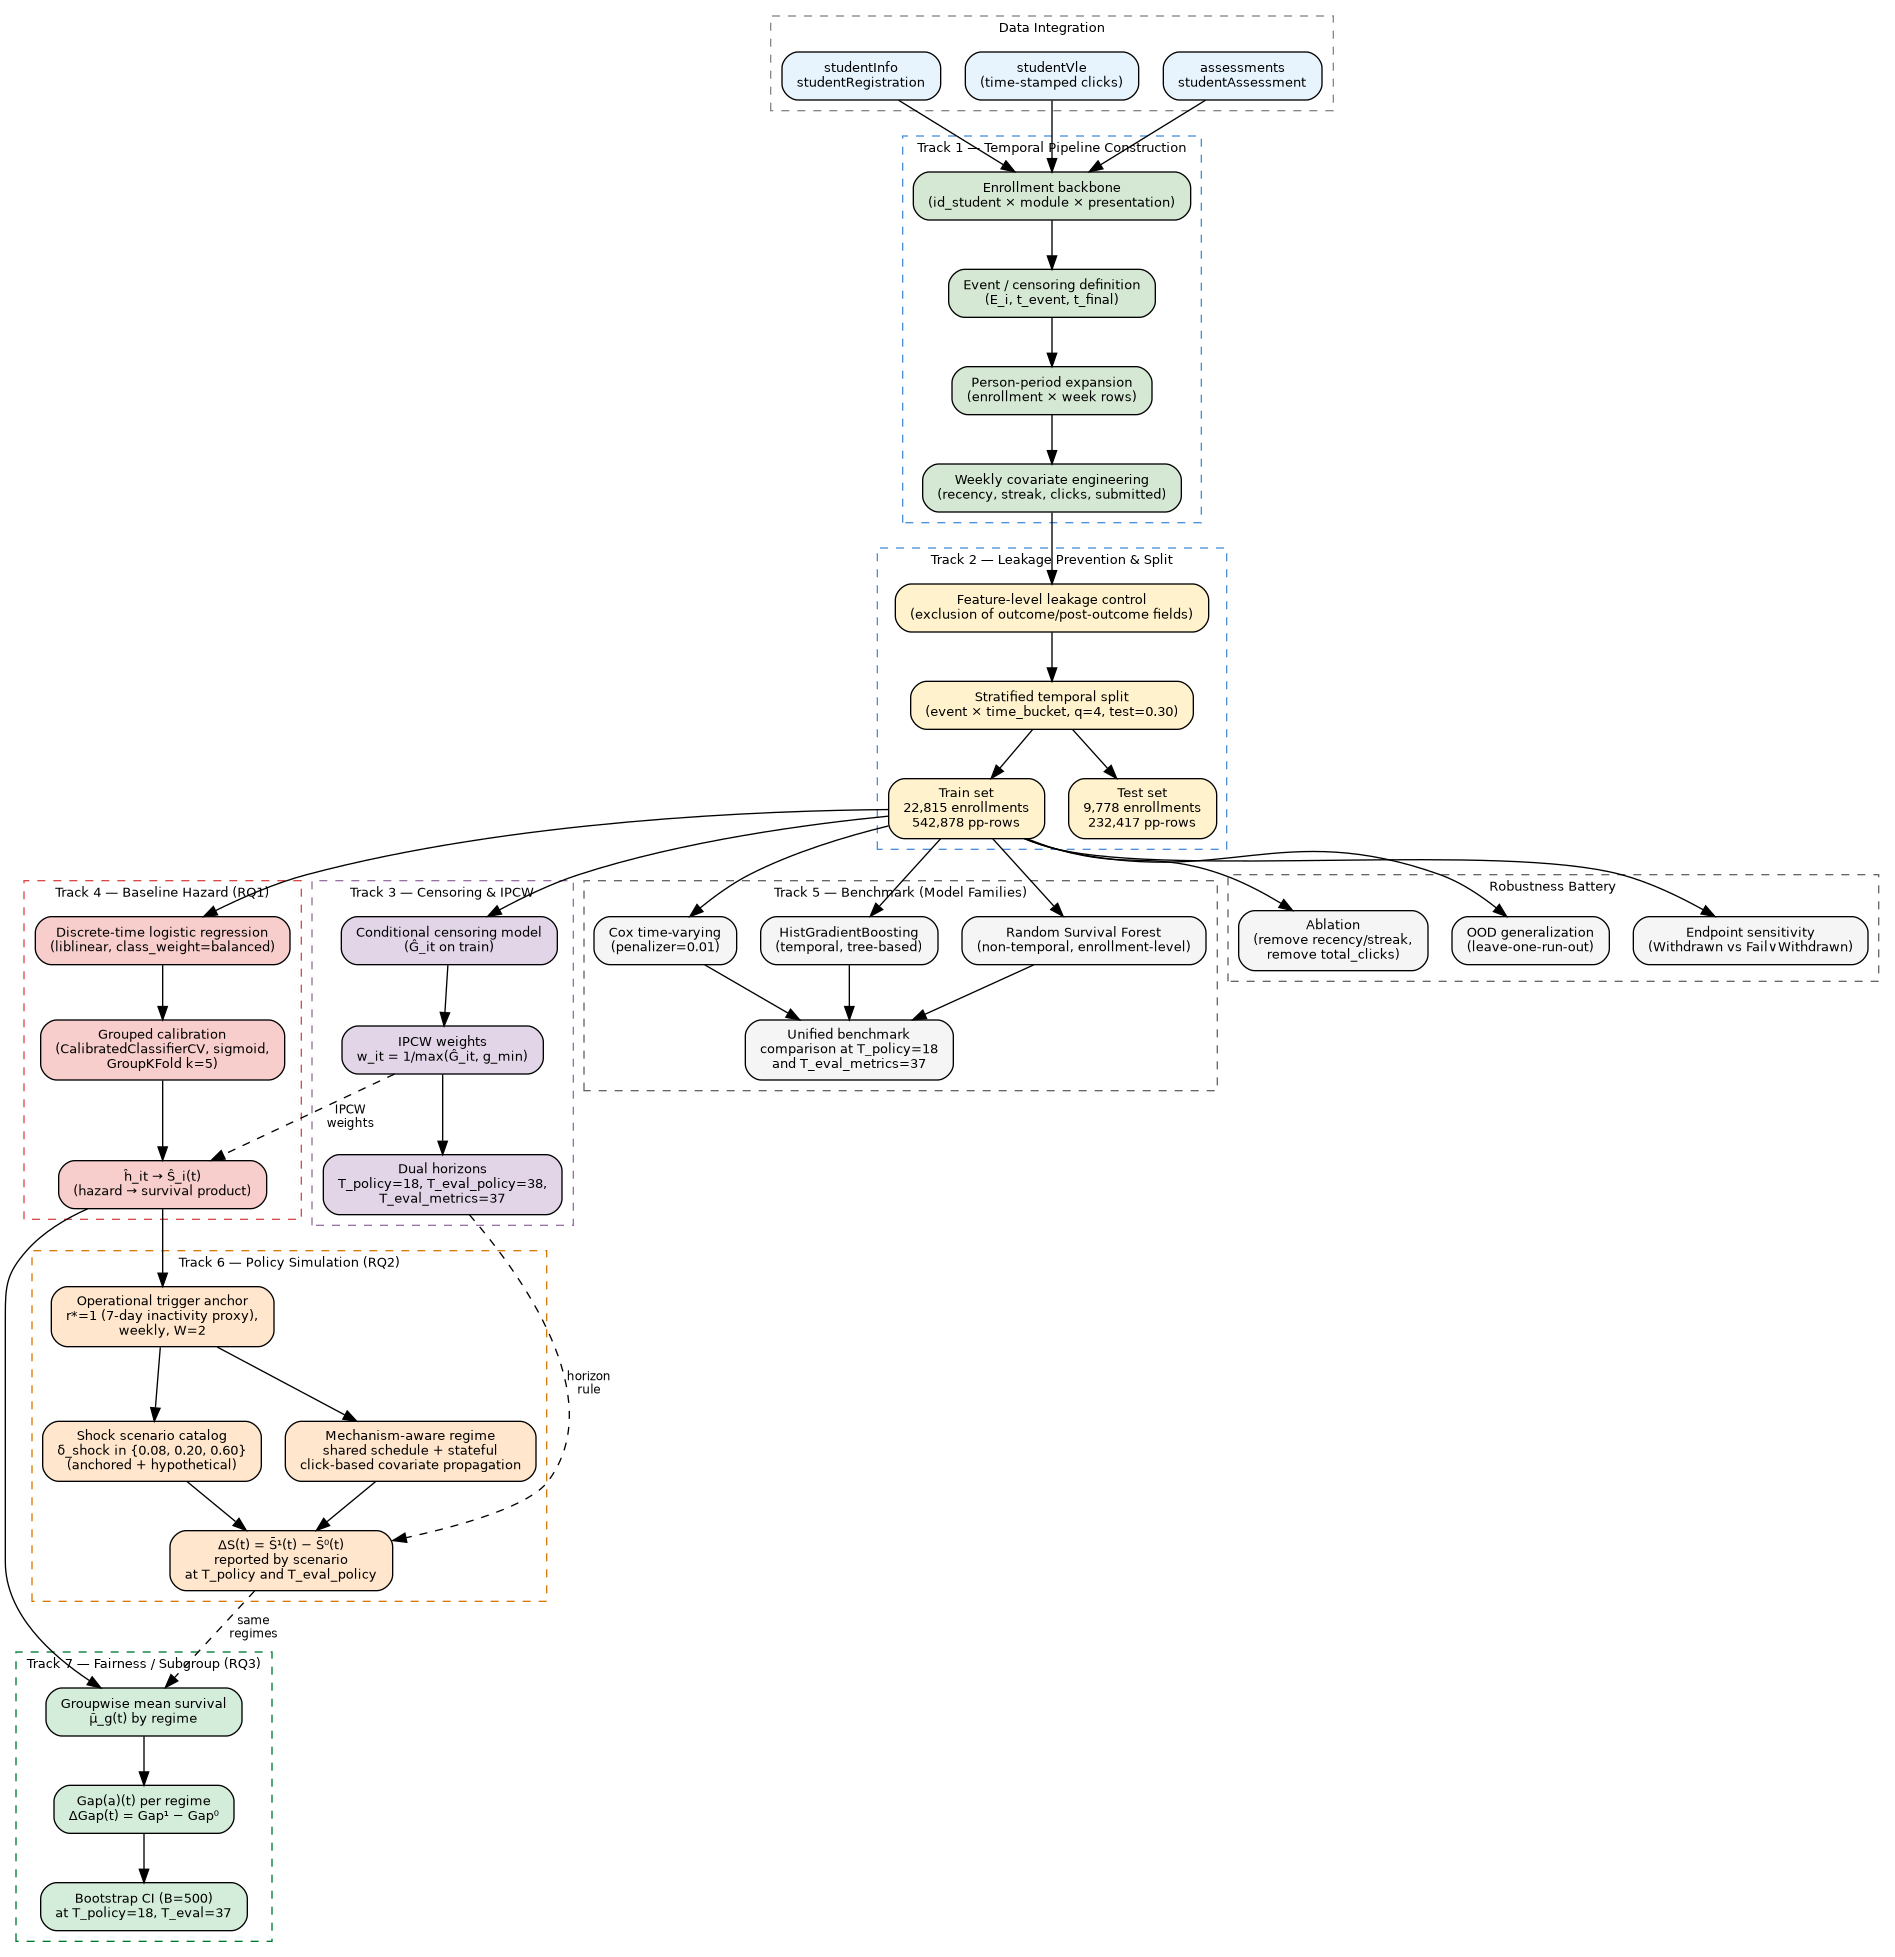
\includegraphics[width=\columnwidth]{figures/fig_pipeline_endtoend.png}
\caption{End-to-end pipeline: data integration, temporal construction, modeling, policy simulation, and fairness evaluation mapped to seven executable tracks and RQ1--RQ3, including dual-horizon semantics ($T_{policy}$, $T_{eval\_policy}$, $T_{eval\_metrics}$) and scenario-indexed shock intensity in RQ2.}
\label{fig:pipeline_endtoend}
\end{figure}

%% -----------------------------------------------------------------------
\subsection{Design Goals and Operational Research Questions}

The experimental design evaluates three core properties of the framework, each aligned with one research question and one analytical track.

\begin{itemize}
\item \textbf{RQ1 --- Temporal hazard quality.}
Does the discrete-time hazard model discriminate and calibrate well enough at the weekly person-period level to support downstream policy evaluation?

\item \textbf{RQ2 --- Structural regime contrast.}
Under an explicit deterministic Recency-triggered rule, does the aggregate structural contrast $\Delta S(t)$ (Eq.~\ref{eq:delta_s}) yield a consistent and interpretable signal at the designated reporting horizons?

\item \textbf{RQ3 --- Subgroup gap change.}
When the same rule is applied to observable subgroups, does $\Delta Gap(t)$ (Eq.~\ref{eq:delta_gap}) exhibit a direction robust to bootstrap uncertainty, thereby motivating subgroup-sensitive support evaluation?
\end{itemize}

These goals define the contract of the section. What is evaluated here is the empirical behavior of the implemented framework under fixed protocol choices. Policy and fairness outputs are therefore interpreted as \textit{simulated regime contrasts}, not as observationally identified causal effects.

%% -----------------------------------------------------------------------
\subsection{Cohort, Unit of Analysis, and Analysis Table}
\label{subsec:cohort}

\paragraph*{Data sources.}
We use the Open University Learning Analytics Dataset (OULAD)~\cite{Kuzilek2017OULAD}, integrating time-stamped VLE interaction logs (\texttt{studentVle}), assessment information (\texttt{assessments}, \texttt{studentAssessment}), and administrative enrollment records (\texttt{studentInfo}, \texttt{studentRegistration}). These sources jointly provide the temporal, assessment, and administrative components required to build a weekly enrollment-level survival dataset.

\paragraph*{Enrollment backbone.}
An enrollment is identified by the triplet $(\texttt{id\_student},\allowbreak\texttt{code\_module},\allowbreak\texttt{code\_presentation})$. After deduplication, the exported cohort contains $N=32{,}593$ enrollments from $28{,}785$ unique students. This enrollment backbone defines the analytical unit used throughout all subsequent tracks.

\paragraph*{Primary endpoint.}
Dropout requires both \texttt{final\_result = Withdrawn} and an observed valid \texttt{date\_unregistration}, yielding the indicator $E_i$ defined in Methodology. Withdrawn records without a valid unregistration date ($2{,}769$ cases) are treated as censored under the primary endpoint. This rule ensures that event counting is restricted to withdrawals with an observed administrative event time compatible with the weekly hazard formulation.

\paragraph*{Person-period table.}
Each enrollment is expanded into weekly rows $t=0,\dots,t_i^{\mathrm{final}}$ with terminal label
\[
event_{it}=\mathbb{1}[E_i=1 \wedge t=t_i^{\mathrm{final}}].
\]
This representation converts the cohort into the person-period structure required for discrete-time hazard estimation and downstream policy simulation. Table~\ref{tab:cohort_summary} reports the resulting cohort dimensions.

\begin{table}[!t]
\centering
\caption{Cohort summary: enrollment and person-period counts.}
\label{tab:cohort_summary}
\begin{tabular}{lr}
\hline
Quantity & Value \\
\hline
Enrollments ($N$) & 32{,}593 \\
Unique students & 28{,}785 \\
Withdrawn without valid date (censored) & 2{,}769 \\
\hline
\end{tabular}
\end{table}

%% -----------------------------------------------------------------------
\subsection{Stratified Temporal Split Protocol}
\label{subsec:split}

The train-test split is performed at the enrollment level to prevent row leakage across weekly observations from the same enrollment. This is a central design choice because the model is trained on person-period rows but evaluated under enrollment-level independence constraints.

\paragraph*{Stratification variable.}
We define
\begin{equation*}
time\_for\_split_i =
\begin{cases}
t_i^{\mathrm{event}}, & \text{if } E_i = 1,\\
t_i^{\mathrm{final}}, & \text{otherwise.}
\end{cases}
\end{equation*}
and then discretize this variable into $q=4$ quantile buckets. The stratum for each enrollment is
\begin{equation*}
stratum_i = (E_i,\; bucket_q(time\_for\_split_i)).
\end{equation*}
Observed bucket edges after rounding are $[0,\;8,\;31,\;34,\;63]$. This design preserves both event-status balance and coarse temporal structure across partitions.

\paragraph*{Sampling.}
Within each stratum, $30\%$ of enrollments are assigned to the test set using random seed 42, with per-stratum count clipped to $[\,1,\; n_s-1\,]$. This guarantees that each populated stratum contributes observations to both train and test whenever possible.

\paragraph*{Resulting partition.}
Table~\ref{tab:split_counts} reports the partition dimensions. All enrollment-weeks associated with a given enrollment appear entirely in train or entirely in test, ensuring that no weekly rows from the same enrollment cross partitions.

\begin{table}[!t]
\centering
\caption{Train/test partition after stratified temporal split.}
\label{tab:split_counts}
\begin{tabular}{lrrr}
\hline
Split & Enrollments & Events & Person-period rows \\
\hline
Train & 22{,}815 & 5{,}171 & 542{,}878 \\
Test  &  9{,}778 & 2{,}216 & 232{,}417 \\
\hline
\end{tabular}
\end{table}

\paragraph*{Validation-level leakage control.}
Calibration and evaluation diagnostics use GroupKFold with $k=5$ folds grouped by the enrollment key. This adds a second layer of protection against leakage by ensuring that no person-period rows from the same enrollment appear in both calibration and validation within a fold.

%% -----------------------------------------------------------------------
\subsection{Model Variants in the Experiment}
\label{subsec:model_variants}

All model variants share the same train-test split and the same leakage controls. Their purpose is not to redefine the primary analysis track, but to situate the main discrete-time hazard model within a controlled comparative design. Table~\ref{tab:model_variants} summarizes their roles.

\begin{table}[!t]
\centering
\footnotesize
\renewcommand{\arraystretch}{1.05}
\caption{Model variants and their roles in the experiment.}
\label{tab:model_variants}
\begin{tabular}{@{}p{0.30\columnwidth} p{0.62\columnwidth}@{}}
\hline
Variant & Role \\
\hline
Discrete-time logistic (primary) &
  Main hazard model. Source of $\hat h_{it}$ and $\hat S_i(t)$ for policy and fairness tracks. \\
HistGradientBoosting (temporal) &
  Tree-based temporal baseline on person-period rows; used in benchmark and ablation packs. \\
Cox time-varying &
  Classical survival benchmark with start--stop weekly intervals~\cite{Cox1972RegressionModels}. \\
Random Survival Forest (non-temporal) &
  Enrollment-level tree-based baseline without weekly trajectory inputs. \\
Unified benchmark pack &
  Standardized comparison of temporal vs.\ non-temporal families at aligned horizons. \\
\hline
\end{tabular}
\end{table}

\paragraph*{Primary model specification.}
The primary model is logistic regression with \texttt{solver=liblinear}, \texttt{max\_iter=4000}, \texttt{class\_weight=balanced}, and \texttt{random\_state=42}. Numeric features (\texttt{total\_clicks}, \texttt{studied\_credits}, \texttt{num\_of\_prev\_attempts}, \texttt{recency}, \texttt{streak}, \texttt{submitted\_this\_week}) are standardized, while categorical variables (\texttt{week}, \texttt{code\_module}, \texttt{code\_presentation}, \texttt{highest\_education}, \texttt{age\_band}, \texttt{gender}) are one-hot encoded with unknown categories ignored. Probability calibration uses \texttt{CalibratedClassifierCV(method=\allowbreak"sigmoid", ensemble=False)} with precomputed GroupKFold splits at the enrollment level. This model is the main source of weekly hazard estimates and reconstructed survival curves.

\paragraph*{Cox time-varying specification.}
The survival benchmark uses \texttt{CoxTimeVaryingFitter} from the \texttt{lifelines} package with \texttt{penalizer=0.01} and start--stop weekly intervals, using numeric covariates available at the weekly level. Its role is to provide a classical survival-analysis reference under the same temporal data construction.

\paragraph*{HistGradientBoosting (temporal diagnostic).}
A \texttt{HistGradientBoostingClassifier} with \texttt{max\_depth=6}, \texttt{learning\_rate=0.05}, \texttt{max\_iter=300}, and \texttt{random\_state=42}, plus ordinal encoding and the same Platt calibration protocol. This tree-based variant operates on person-period rows and is used in the benchmark and ablation packs to verify that the main conclusions are not specific to the logistic model family.

\paragraph*{Non-temporal baseline (Random Survival Forest).}
A Random Survival Forest from the \texttt{scikit-survival} package (with classification fallback when needed) estimating $\hat p_i^{(T)}=1-\hat S_i(T)$ from enrollment-level static features only, without weekly trajectory inputs. It is evaluated at $T_{policy}$ and $T_{eval\_metrics}$ to isolate the contribution of the temporal person-period structure.

%% -----------------------------------------------------------------------
\subsection{Evaluation Horizons and Stability Rule}
\label{subsec:horizons}

Because censoring support deteriorates over time, late-horizon evaluation requires explicit stability rules. The design therefore separates two evaluation perspectives, one substantive and one technical, each tied to a different horizon rule (Figure~\ref{fig:censoring_dual_horizons}).

% Placeholder for compiled Graphviz figure (G3 censoring_dual_horizons)
% To produce: dot -Tpng graphviz_censoring_dual_horizons.txt -o figures/fig_censoring_dual_horizons.png
\begin{figure}[!t]
\centering
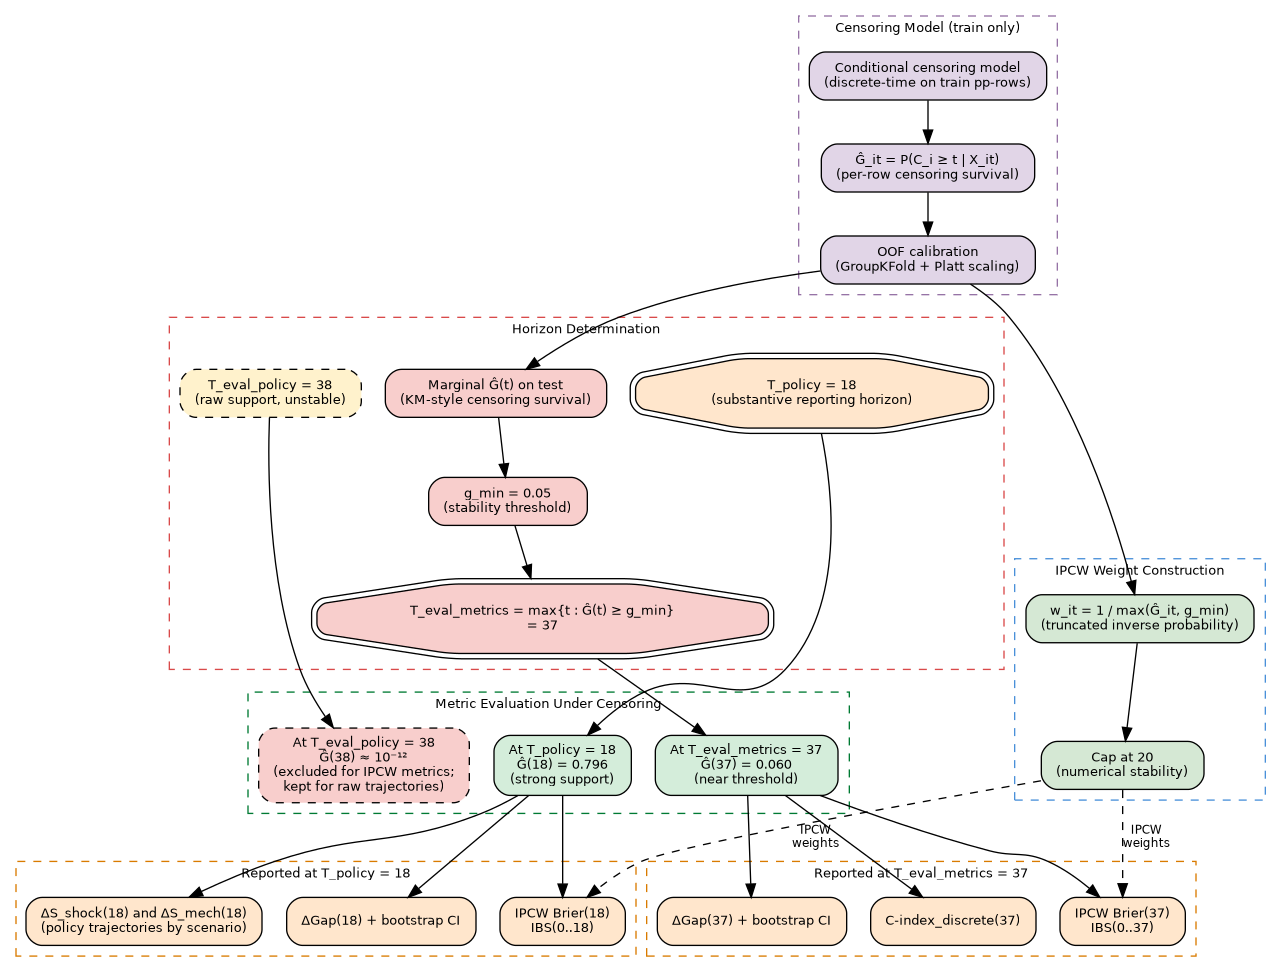
\includegraphics[width=\columnwidth]{figures/fig_censoring_dual_horizons.png}
\caption{Censoring-aware evaluation flow: the conditional censoring model determines IPCW weights and horizon stability, separating $T_{eval\_metrics}=37$ for weighted metrics from $T_{eval\_policy}=38$ for raw policy trajectories, with $T_{policy}=18$ as the substantive reporting horizon.}
\label{fig:censoring_dual_horizons}
\end{figure}

\paragraph*{Policy reporting horizon.}
$T_{policy}=18$ is the substantive horizon at which aggregate $\Delta S$ and subgroup $\Delta Gap$ are primarily reported. At this horizon, censoring survival is $\hat G(18)=0.796$, indicating strong support for IPCW-based summaries.

\paragraph*{Technical metric horizon.}
The stable IPCW horizon is
\begin{equation*}
T_{eval\_metrics}=\max\{t:\hat G(t)\ge g_{min}\},
\end{equation*}
with $g_{min}=0.05$, yielding $T_{eval\_metrics}=37$ and $\hat G(37)=0.060$. Beyond this point, $\hat G(38)\approx 10^{-12}$, making IPCW-based summaries numerically unstable. This horizon is therefore used as the last reliable point for weighted metric reporting.

\paragraph*{Raw support horizon.}
$T_{eval\_policy}=38$ denotes the maximum observed test support. It is retained for trajectory visualization only and is explicitly excluded from quantitative IPCW-based reporting.

\paragraph*{Censoring model.}
A conditional discrete-time model is fit on training person-period rows to estimate $\hat G_{it}=P(C_i\ge t \mid X_{it})$. Stabilized IPCW weights are defined as
\[
w_{it}=1/\max(\hat G_{it},\,g_{min}),
\]
and capped at 20 for numerical stability. Out-of-fold calibration is performed via GroupKFold plus Platt scaling. Together, these choices define the technical support conditions under which weighted metrics are reported.

%% -----------------------------------------------------------------------
\subsection{Primary and Secondary Metrics}
\label{subsec:metrics}

The metric suite is designed to distinguish discrimination, calibration, and horizon-specific predictive quality. Table~\ref{tab:metric_suite} maps each metric to the question it addresses and the horizon at which it is reported.

\begin{table}[!t]
\centering
\footnotesize
\renewcommand{\arraystretch}{1.05}
\caption{Evaluation metric suite and reporting horizons.}
\label{tab:metric_suite}
\begin{tabular}{@{}p{0.26\columnwidth} p{0.32\columnwidth} p{0.30\columnwidth}@{}}
\hline
Metric & Question addressed & Horizon(s) \\
\hline
$AUC_{row}$ &
  Row-level hazard discrimination &
  Full test support \\
IPCW Brier$(T)$ &
  Calibration at horizon $T$ &
  $T_{policy}$, $T_{eval}$ \\
IBS$(0{:}T)$ &
  Integrated calibration up to $T$ &
  $T_{policy}$, $T_{eval}$ \\
C-index$_{discrete}(T)$ &
  Ranking of event-time pairs &
  $T_{policy}$, $T_{eval}$ \\
ECE (15 bins) &
  Binned calibration error &
  Full test support \\
\hline
\end{tabular}
\end{table}

\paragraph*{Row-level AUC.}
AUC is computed on person-period test rows using target $event_{it}$ and score $\hat h_{it}$. Because the evaluation unit is the person-period row, this metric diagnoses row-level hazard discrimination rather than static enrollment-level classification performance.

\paragraph*{IPCW Brier score.}
Event probability at horizon $T$ is $\hat p_i^{(T)}=1-\hat S_i(T)$, with horizon label
\[
Y_i^{(T)}=\mathbb{1}\{E_i=1,\;t_i^{\mathrm{event}}\le T\}.
\]
The censoring-weighted Brier score~\cite{Graf1999AssessmentSurvivalPrediction} is
\begin{equation*}
BS_{IPCW}(T)=\frac{1}{n}\sum_i w_i(T)\left(Y_i^{(T)}-\hat p_i^{(T)}\right)^2.
\end{equation*}
This quantity evaluates horizon-specific probabilistic accuracy under censoring-aware weighting.

\paragraph*{Integrated Brier Score (IBS).}
\begin{equation*}
IBS(0{:}T)=\frac{1}{T+1}\sum_{t=0}^{T}BS_{IPCW}(t).
\end{equation*}
IBS summarizes calibration quality over an interval rather than at a single horizon, making it useful for comparing models over a span of weeks rather than at one fixed time point.

%% -----------------------------------------------------------------------
\subsection{Policy Evaluation Protocol (RQ2)}
\label{subsec:policy_eval}

The policy track compares two simulated regime constructions under the same deterministic trigger. This keeps the intervention rule fixed while isolating differences in how the regime is propagated through the model.

\paragraph*{Scenario specification.}
Table~\ref{tab:policy_spec} records the operational intervention anchor, and Table~\ref{tab:policy_intensity} records scenario-intensity assumptions. This separation makes explicit what is externally anchored versus what is treated as a simulation hypothesis.

\begin{table}[!t]
\centering
\caption{Operational intervention anchor (RQ2).}
\label{tab:policy_spec}
\begin{tabular}{lr}
\hline
Parameter & Value \\
\hline
$r^*$ (weekly proxy for 7-day inactivity) & 1 \\
Trigger frequency & weekly \\
$W$ (active window length) & 2 \\
Intervention class & short-term digital nudge \\
Anchor source & Kay \& Bostock (2023) \\
\hline
\end{tabular}
\end{table}

\begin{table}[!t]
\centering
\caption{Scenario-intensity assumptions for shock and shared mechanism-aware schedule (RQ2).}
\label{tab:policy_intensity}
\begin{tabular}{llp{0.53\columnwidth}}
\hline
Component & Value(s) & Interpretation \\
\hline
$\delta_{shock}$ & 0.08 & anchored conservative (qualitative anchor: Sneyers \& De Witte \cite{SneyersDeWitte2018InterventionsMeta}) \\
$\delta_{shock}$ & 0.20 & hypothetical A (legacy baseline) \\
$\delta_{shock}$ & 0.60 & hypothetical B (stress test) \\
$\alpha_{week0}$ & 0.35 & shared mechanism-aware schedule parameter \\
$\alpha_{week1}$ & 0.10 & shared mechanism-aware schedule parameter \\
Decay type & kb2023\_step\_2w & shared mechanism-aware schedule parameter \\
Window upper bound & exclusive & shared mechanism-aware schedule parameter \\
\hline
\end{tabular}
\end{table}

Operationally, the trigger and intervention class are anchored to Kay and Bostock \cite{KayBostock2023PowerNudge}, while shock intensity is treated as a scenario hypothesis under observational non-identification. The conservative scenario ($\delta_{shock}=0.08$) is anchored qualitatively, and the higher intensities are explicit hypothetical stress settings.

\paragraph*{Regimes compared.}
\begin{enumerate}
\item \textbf{Baseline regime ($a=0$):}
observed hazard trajectory $\hat h_{it}^{(0)}$.

\item \textbf{Shock regime ($a=1$, shock):}
hazard scaled by $(1-\delta_{shock,s})$ within active weeks, where $s$ indexes the scenario catalog.

\item \textbf{Mechanism-aware regime ($a=1$, mech):}
covariates overwritten within active weeks (click-based engagement boosted by schedule factor, activity/recency/streak propagated statefully), then hazard recomputed via plug-in prediction. The click perturbation is an LMS proxy analogous to participation/re-engagement dynamics in Kay and Bostock (2023), not a literal variable-level replication.
\end{enumerate}

Event rows are forced inactive in all regimes to prevent post-event counterfactual contamination. This rule ensures that counterfactual propagation only affects weeks in which the enrollment remains under risk.

\paragraph*{Outputs reported.}
For each regime, survival is reconstructed via the discrete-time product, and the aggregate structural contrast is
\[
\Delta S(t)=\bar S^{(1)}(t)-\bar S^{(0)}(t).
\]
Primary reporting for policy trajectories focuses on $\Delta S(T_{policy})$ and $\Delta S(T_{eval\_policy})$ by scenario; censoring-weighted metric diagnostics remain tied to $T_{eval\_metrics}$. These outputs provide the central empirical evidence for RQ2 under the interpretive contract of simulated regime comparison.

%% -----------------------------------------------------------------------
\subsection{Subgroup Evaluation Protocol (RQ3)}
\label{subsec:fairness_eval}

This track evaluates whether the same policy produces a differential change in outcome trajectories across observable groups, while preserving the same modeling and simulation engine used in the aggregate analysis.

\paragraph*{Demonstration variable.}
The fairness track uses \texttt{gender} as an operational demonstration variable with $g(i)\in\{0,1\}$. The framework itself is group-agnostic: the same protocol can be applied to any observable subgroup definition available in the dataset.

\paragraph*{Evaluated quantities.}
Under each regime $a\in\{0,1\}$, the following quantities are computed:
\begin{itemize}
\item groupwise mean survival $\bar\mu_g^{(a)}(t)$;
\item regime-specific gap $Gap^{(a)}(t)=\bar\mu_1^{(a)}(t)-\bar\mu_0^{(a)}(t)$;
\item change-in-gap $\Delta Gap(t)=Gap^{(1)}(t)-Gap^{(0)}(t)$.
\end{itemize}
All quantities are reported at both $T_{policy}=18$ and $T_{eval\_metrics}=37$. This mirrors the dual-horizon logic used in the aggregate policy track.

\paragraph*{Uncertainty via bootstrap.}
A total of $B=500$ bootstrap resamples with seed 42 are used to construct $95\%$ confidence intervals for $\Delta Gap(T)$. The reading rule is:
if $0\notin CI_{95\%}(\Delta Gap(T))$, the direction of gap change is considered robust at horizon $T$. This criterion provides an uncertainty-aware interpretation rather than relying on point estimates alone.

\paragraph*{Predictive fairness diagnostics.}
By-group row-level metrics (AUC, Brier, and ECE with 15 bins) and calibration curves are reported on test rows. Their role is to verify that subgroup-level policy contrasts are not being interpreted on top of severely asymmetric predictive quality across groups.

%% -----------------------------------------------------------------------
\subsection{Planned Robustness Battery}
\label{subsec:robustness}

The robustness plan was defined before examining comparative outcomes. Its purpose is to probe whether the main conclusions are sensitive to feature dependence, domain shift, or endpoint specification (Figure~\ref{fig:benchmark_robustness}).

% Placeholder for Graphviz figure (G4 benchmark_robustness)
% To produce: dot -Tpng graphviz_benchmark_robustness.txt -o figures/fig_benchmark_robustness.png
\begin{figure}[!t]
\centering
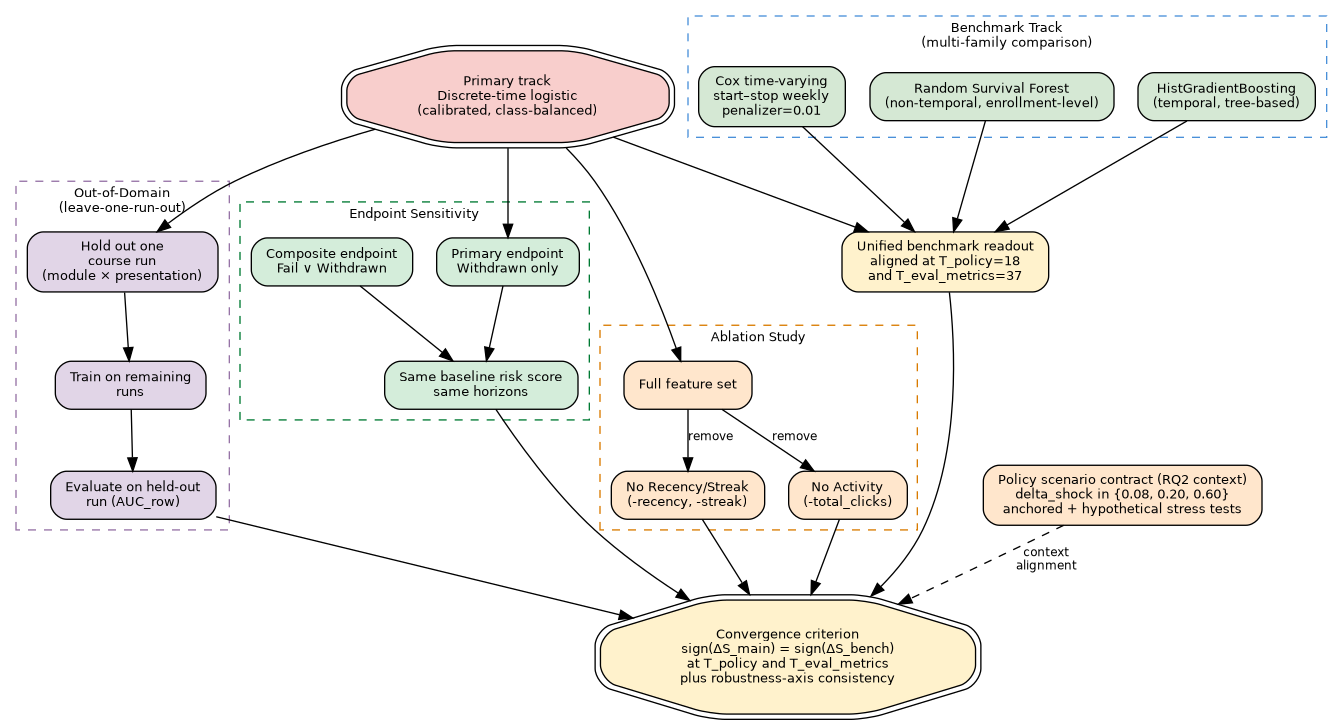
\includegraphics[width=\columnwidth]{figures/fig_benchmark_robustness.png}
\caption{Benchmark and robustness battery: the primary model is compared against alternative families (benchmark), feature subsets (ablation), unseen course runs (OOD), and an alternative endpoint (sensitivity), with convergence read at $T_{policy}$ and $T_{eval\_metrics}$ and interpreted under the scenario-aware RQ2 policy contract.}
\label{fig:benchmark_robustness}
\end{figure}

\paragraph*{Ablation study.}
Three model variants are retrained under the same protocol:
\begin{enumerate}
\item \textbf{Full:} all features;
\item \textbf{No Recency/Streak:} drops \texttt{recency} and \texttt{streak};
\item \textbf{No Activity:} drops \texttt{total\_clicks}.
\end{enumerate}
Each variant is retrained with
\texttt{LogisticRegression} with \texttt{solver="liblinear"},
\texttt{max\_iter=2000}, \texttt{class\_weight="balanced"}, and
\texttt{random\_state=42}
plus the same Platt calibration protocol. The leakage guard excludes all outcome and post-outcome fields. Metrics reported are $AUC_{row,test}$, $C\text{-index}_{discrete}(T_{eval})$, $BS_{IPCW}(T_{eval})$, and $IBS(0{:}T_{eval})$. This axis tests how dependent the main conclusions are on the core temporal engagement features.

\paragraph*{Out-of-domain generalization (leave-one-run-out).}
One entire course run $(\texttt{code\_module},\texttt{code\_presentation})$ is held out from training and used as the sole test set. The model is retrained on the remaining runs and evaluated via $AUC_{row}$ on the held-out person-period rows. Five held-out runs are reported to expose course-run heterogeneity and assess how far the main hazard model generalizes beyond pooled training conditions.

\paragraph*{Endpoint sensitivity.}
The primary endpoint is Withdrawn with valid unregistration date. As a sensitivity check, a composite endpoint (\textit{Fail} $\lor$ \textit{Withdrawn}) is evaluated using the \emph{same baseline risk score} $1-\hat S(t)$ produced by the model trained on the primary endpoint. For Fail cases, which lack an administrative unregistration date in OULAD, a terminal-time proxy based on the final observed week is used. Metrics are compared at the same horizons ($T_{policy}$, $T_{eval\_metrics}$). This sensitivity analysis tests whether the reading of results is materially altered by a broader operational endpoint.

%% -----------------------------------------------------------------------
\subsection{Comparison Rules and Reading Criteria}
\label{subsec:reading_criteria}

This subsection states explicitly how competing empirical signals are read. Its role is to prevent post hoc interpretation drift by fixing the directional rules used in comparative analysis.

\paragraph*{Sign consistency across families.}
The primary convergence check requires that the direction of $\Delta S$ be consistent between the main model and benchmarks:
\begin{equation*}
\mathrm{sign}\!\left(\Delta S_{main}(T)\right)
= \mathrm{sign}\!\left(\Delta S_{benchmark}(T)\right).
\end{equation*}
This rule does not require identical magnitudes across families; it requires agreement in the directional conclusion.

\paragraph*{Sign consistency in fairness.}
A fairness signal is considered robust when
\begin{equation*}
0 \notin CI_{95\%}\!\left(\Delta Gap(T)\right).
\end{equation*}
This criterion translates bootstrap uncertainty into a binary robustness reading for subgroup gap change at the reporting horizon.

\paragraph*{Stability across robustness axes.}
For each robustness axis $r$ (ablation, OOD, endpoint), robustness is assessed by directional stability:
\begin{equation*}
\mathrm{sign}\!\left(\Delta S_r(T)\right)
= \mathrm{sign}\!\left(\Delta S_{main}(T)\right),
\end{equation*}
while the spread within each axis is used as a sensitivity diagnostic. In this way, robustness is defined as preservation of the substantive conclusion under controlled design perturbations.

%% -----------------------------------------------------------------------
\subsection{Evidence Contract and Artifact Traceability}
\label{subsec:artifacts}

This subsection defines how empirical claims are tied to concrete outputs. It establishes the section's evidence contract and makes explicit the traceability expectations that later govern the Results section.

\paragraph*{Claim-to-evidence mapping.}
Every claim in Results must satisfy
\begin{equation*}
claim_j \;\rightarrow\; \{metric_j,\; figure_k,\; table_m,\; horizon_h\},
\end{equation*}
where figures and tables correspond to exported artifacts under \texttt{outputs\_v2/figures/} and \texttt{outputs\_v2/tables/}. This rule ensures that every interpretive statement can be audited back to a specific metric, artifact, and reporting horizon.

\paragraph*{Main text vs.\ appendix.}
The main text includes only evidence essential to the central argument, namely calibration, $\Delta S$, $\Delta Gap$, and benchmark convergence. Extended diagnostics, including per-group calibration curves, covariate delta profiles, and bootstrap histograms, are placed in the appendix. This separation keeps the main narrative focused while preserving auditability.

\paragraph*{Reproducibility.}
The complete pipeline---preprocessing, split generation, training and calibration, policy simulation, fairness diagnostics, and artifact export---is available at
\url{https://github.com/rafa-rodriguess/TCM-Student-Dropout}
\cite{RafaRepoTCMStudentDropout}. Horizon parameters ($T_{policy}$, $T_{eval\_policy}$, $T_{eval\_metrics}$, $g_{min}$), policy specification ($r^*$, $W$, shared mechanism-aware schedule, and scenario-indexed $\delta_{shock}$), and random seeds are recorded in the pipeline source. The scenario contract is exported in \nolinkurl{table_policy_scenarios_main.csv} and \nolinkurl{table_policy_scenario_params.csv}, with trajectory outputs exported in \nolinkurl{table_policy_deltaS_by_week_by_scenario.csv} and \nolinkurl{table_policy_deltaS_at_horizons_by_scenario.csv}. This traceability layer links the formal protocol described here to the executable notebook and exported evidence package.

%% -----------------------------------------------------------------------
\subsection{Executable Pipeline Summary}

Algorithm~\ref{alg:pipeline} summarizes the end-to-end executable pipeline from data integration through fairness evaluation. Its purpose is not to introduce new methodology, but to condense the protocol into a single operational sequence consistent with the previous subsections.

\begin{algorithm}[!t]
\caption{Discrete-Time Survival + Counterfactual Policy Simulation}
\label{alg:pipeline}
\small
\begin{algorithmic}[1]
\Require OULAD tables: \texttt{studentInfo}, \texttt{studentRegistration}, \texttt{studentVle}
\Ensure $\hat S^{(0)}(t)$, $\hat S^{(1)}(t)$, $\Delta S(T_{policy})$, $\Delta Gap(T)$ with bootstrap CI, exported artifacts

\State Build enrollment backbone keyed by $(\texttt{id\_student},\texttt{code\_module},\texttt{code\_presentation})$.
\State Define endpoint: $E_i=\mathbb{1}[\texttt{Withdrawn} \wedge \texttt{date\_unregistration valid}]$; $t^{event}_i=\lfloor \texttt{date\_unregistration}/7 \rfloor$.
\State Compute censoring anchor $t^{last}_i$ (last observed week with non-negative VLE activity; default 0).
\State Define $t^{final}_i$: $t^{event}_i$ if $E_i=1$; $t^{last}_i$ otherwise.
\State Construct weekly person-period rows $t=0,\dots,t^{final}_i$ with $event_{it}=\mathbb{1}[E_i=1 \wedge t=t^{final}_i]$.
\State Engineer weekly covariates $X_{it}$ (clicks, Recency, Streak, submitted) using $w(d)=\max(\lfloor d/7\rfloor,0)$.
\State Perform enrollment-stratified temporal split with $q=4$ buckets and \texttt{test\_size}=0.30.
\State Fit the discrete-time hazard model on training rows (penalized, class-balanced logistic + sigmoid calibration).
\State Compute $\hat h^{(0)}_{it}$ on test rows; reconstruct $\hat S^{(0)}_i(t)=\prod_{k\le t}(1-\hat h^{(0)}_{ik})$.
\State Apply the Recency-triggered policy ($r^*=1$, $W=2$) under scenario catalog $\delta_{shock}\in\{0.08,0.20,0.60\}$:
\State \hspace{6pt} \textit{Shock:} $\hat h^{(1,shock,s)}_{it}=\hat h^{(0)}_{it}(1-\delta_{shock,s})$ when active.
\State \hspace{6pt} \textit{Mechanism-aware:} overwrite covariates in the active window (primarily click-based engagement), propagate statefully, and recompute $\hat h^{(1,mech)}_{it}=f(X^{cf}_{it})$.
\State Compute $\hat S^{(1)}_i(t)$ for each regime and scenario; report $\Delta S(T_{policy})$ and $\Delta S(T_{eval\_policy})$ by scenario.
\State Report diagnostics: $AUC_{row}$, $BS_{IPCW}$, and IBS at both horizons.
\State Perform subgroup validation (RQ3): compute $\bar\mu^{(a)}_g(t)$, $Gap^{(a)}(t)$, and $\Delta Gap(t)$ at $T_{policy}=18$ and $T_{eval}=37$.
\State \hspace{6pt} Summarize subgroup uncertainty using $B=500$ bootstrap confidence intervals.
\end{algorithmic}
\end{algorithm}

%% -----------------------------------------------------------------------
\subsection{Limits of the Experimental Design}
\label{subsec:design_limits}

The experimental design evaluates temporal predictive quality and structural regime contrasts under explicit protocol rules; it does not constitute a causal identification design for intervention effects. These limits are part of the section's interpretive contract and should be read together with the evidence rules defined above.

Specifically:
\begin{itemize}
\item Policy and fairness results are \textit{model-implied simulated regime contrasts} under fixed scenario parameters, not observationally identified effects.
\item The censoring treatment uses IPCW for evaluation diagnostics, but it does not apply censoring-weighted retraining or pursue causal identification strategies for potentially informative censoring.
\item Out-of-domain generalization is evaluated via leave-one-run-out, but the pooled training strategy does not explicitly model instructional heterogeneity across course runs.
\item The endpoint sensitivity analysis does not impute event times for Fail cases; instead, it uses a terminal-time proxy based on the final observed week because OULAD does not provide an administrative withdrawal timestamp for Fail.
\end{itemize}

These boundaries define what the reader should and should not infer from the results. The section promises a transparent, pre-specified, and executable evaluation design for temporal prediction, regime comparison, and subgroup diagnostics; it does not promise causal effect estimation from observational exposure.